\documentclass[12pt, a4papre]{article}
\usepackage[catalan]{babel}
\usepackage[unicode]{hyperref}
\usepackage{amsmath}
\usepackage{amssymb}
\usepackage{amsthm}
\usepackage{xifthen}
\usepackage{siunitx}
\usepackage{xcolor}
\usepackage{float}
\usepackage{listings}
\usepackage{setspace}
\usepackage{graphicx}
\usepackage{tikz,lipsum,lmodern}
\usepackage[most]{tcolorbox}
\usepackage{circuitikz}
\usepackage{indentfirst}
\usepackage{verbatimbox}
\usepackage[T1]{fontenc}
\usepackage{beramono}% monospaced font with bold variant
 \usepackage{tikz-timing}[2009/05/15]
\usepackage{listings}
\lstdefinelanguage{VHDL}{
   morekeywords={
     library,use,all,entity,is,port,in,out,end,architecture,of,
     begin,and
   },
   morecomment=[l]--
}
 
\usepackage{xcolor}
\colorlet{keyword}{blue!100!black!80}
\colorlet{comment}{green!50!black!90}
\lstdefinestyle{vhdl}{
   language     = VHDL,
   basicstyle   = \ttfamily,
   keywordstyle = \color{keyword}\bfseries,
   commentstyle = \color{comment}
}

\graphicspath{ {./Imatges/} }


\newcommand{\norm}[1]{\lvert #1 \rvert}

\hypersetup{
    colorlinks = true,
    linkcolor = blue
}

\author{Daniel Vilardell\\
	   Igor Yuziv}
\title{Previ DGD practica 3}
\date{}

\begin{document}
	\maketitle

	1.- Proposeu una descripció VHDL d’un comptador BCD de dues xifres, amb entrada
síncrona d’habilitació de compte i reset asíncron.

	\begin{lstlisting}[style=vhdl, frame=single, basicstyle=\tiny]
	
library ieee;
use ieee.std_logic_1164.all;
use ieee.std_logic_signed.all;

entity comptadorBCD is
	port (nrst, clk, ecnt : in std_logic;
		numx : out std_logic_vector(7 downto 0));
end comptadorBCD;

architecture compte of comptadorBCD is 
	signal unitats, desenes : std_logic_vector (3 downto 0);
	
begin 
	process(clk, nrst)
	begin
	    if nrst = '0' then desenes <= "0000";
			unitats <= "0000";
	    elsif clk' event and clk='1' then
		if ecnt = '1' then
		if desenes = "1001" and unitats = "1001" then desenes <= "0000";
			unitats <= "0000";
		elsif unitats = "1001" then desenes <= desenes +1;
			unitats <= "0000";
		else unitats <= unitats+1;
		end if;
	    end if;
	end if;
end process;
numx (7 downto 4) <= desenes;
numx (3 downto 0) <= unitats;

end compte;
\end{lstlisting}


2.- Proposeu una descripció VHDL del bloc comparador

	\begin{lstlisting}[style=vhdl, frame=single, basicstyle=\tiny]
	
library ieee;
use ieee.std_logic_1164.all;

entity comparadorBCD is 
	port (numx,num : in std_logic_vector (7 downto 0);
			ngtx,nltx,netx: out std_logic);
end comparadorBCD;

architecture comparador of comparadorBCD is 
	begin
	ngtx <= '1' when num > numx else '0';
	netx <= '1' when num = numx else '0';
	nltx <= '1' when num < numx else '0';
end comparador;
	
	\end{lstlisting}
	
	3.- Expliqueu, omplint el cronograma proposat, quin ha de ser el funcionament de la
màquina d’estats control. Dibuixeu el seu diagrama d’estats. Recordeu que ha de ser
del tipus Mealy.

\begin{figure}[H]
		\begin{center}
		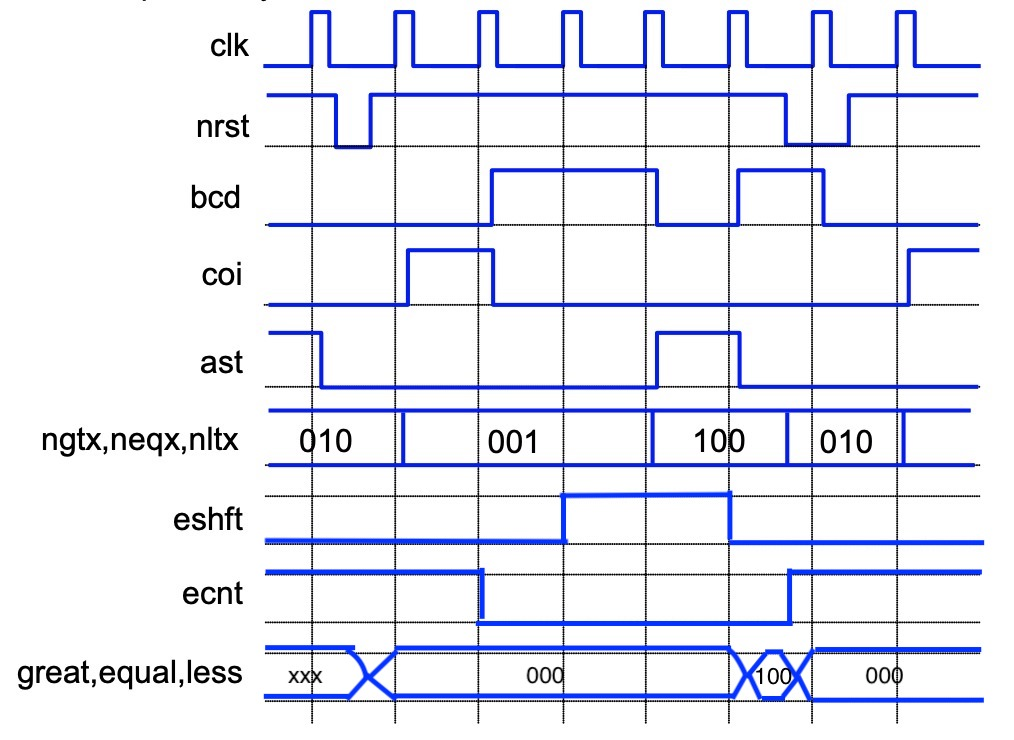
\includegraphics[width=130mm]{pregunta3.jpeg}
		\end{center}
	\end{figure}
	
	\begin{figure}[H]
		\begin{center}
		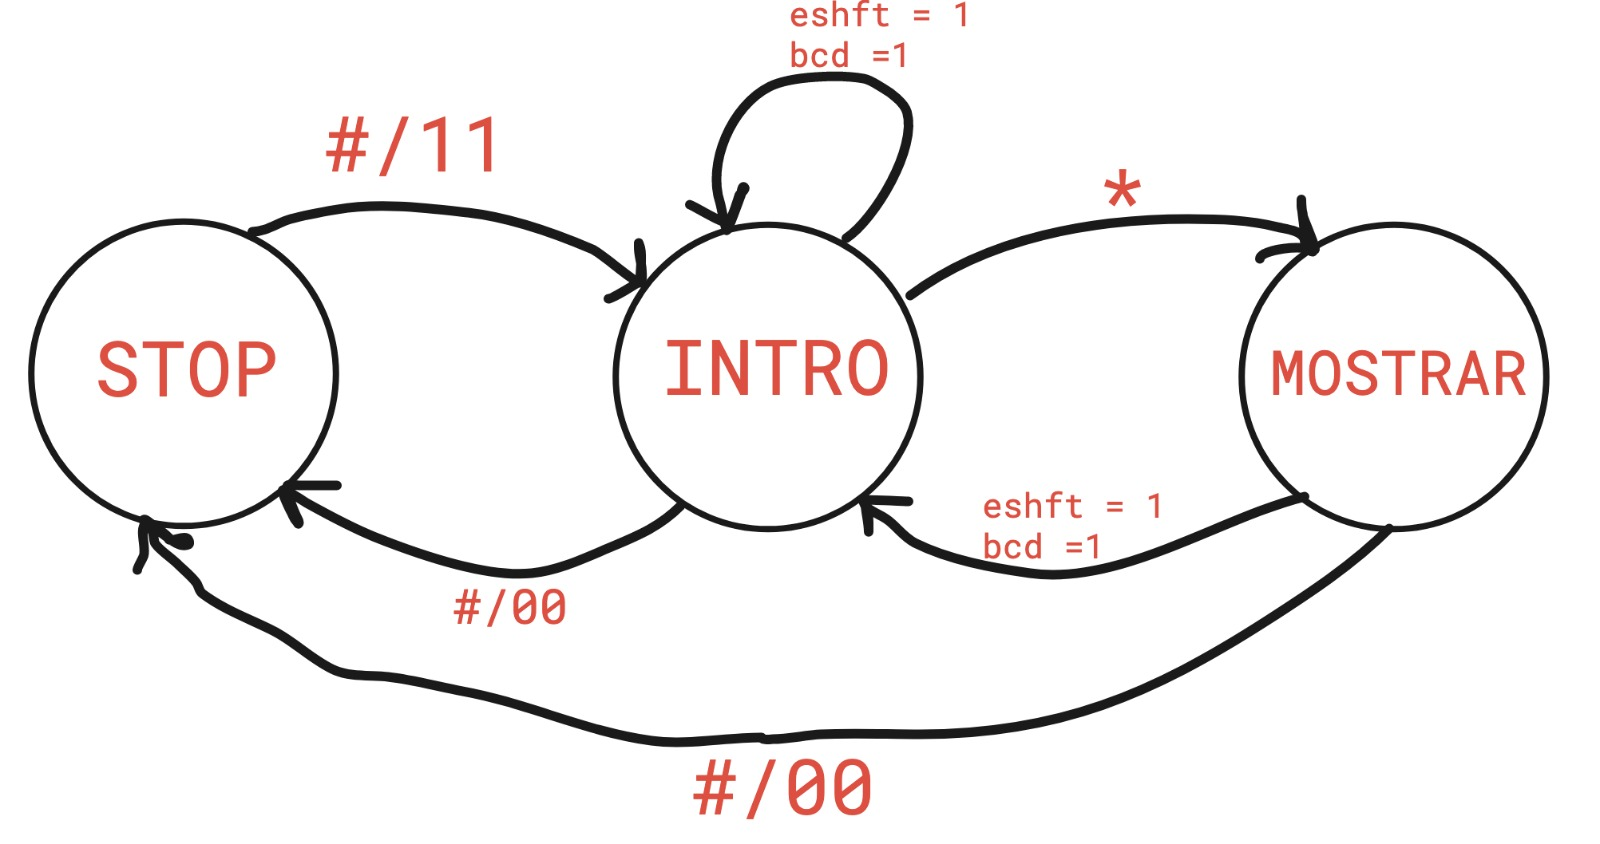
\includegraphics[width=130mm]{diagramadeestats.jpeg}
		\end{center}
	\end{figure}
	
4.- Proposeu una descripció VHDL de la màquina d’estats control.

\begin{lstlisting}[style=vhdl, frame=single, basicstyle=\tiny]
library ieee;
use ieee.std_logic_1164.all;

entity control is
	port (nrst,clk,bcd,ast,coi,ngtx,netx,nltx : in std_logic;
		ecnt, eshft : out std_logic;
		led : out std_logic_vector(7 downto 0));
	end control;

architecture arcControl of control is 
	type maquina is (inicial, intro_data, mostrar_resultat);
	signal estat: maquina;
begin
	process(clk, nrst) begin
	if nrst = '0' then estat <= inicial;
	elsif clk'event and clk ='1' then
	    case estat is 
	    when inicial => if ast = '1' then estat <= intro_data; end if;
	    when intro_data => if coi = '1' and ast = '0' then estat <= mostrar_resultat;
		elsif ast = '1' and coi = '0' then estat <= inicial;
		end if;
	    when mostrar_resultat => if ast = '1' then estat <= inicial;
		elsif netx = '1' then estat <= mostrar_resultat;
		elsif bcd = '1' then estat <= intro_data;
		end if;
	    end case;
	end if;
end process;

ecnt <= '1' when estat = inicial else '0';
eshft <= '1' when (estat = intro_data and bcd = '1') or
			(estat = mostrar_resultat and netx = '0' and bcd = '1') else '0';
			
led <= "11111111" when estat = inicial 
    else "11110000" when estat = mostrar_resultat and nltx = '1' 
        and netx= '0' and ngtx = '0'
    else "00111100" when estat = mostrar_resultat and netx = '1' 
    	and nltx = '0' and ngtx = '0'
    else "00001111" when estat = mostrar_resultat and ngtx = '1' 
    	and nltx = '0' and netx = '0'
    else "00000000";
end arcControl;	
\end{lstlisting}
		
		
	
\end{document}